% !TeX root = ../../paper.tex
\subsection{Alpha-Beta-Suche} \label{ch:alpha-beta-pruning}

Bedenkzeit ist im Wettbewerbsschach eine begrenzte Ressource.
Deshalb muss sowohl die Güte eines Schachspielers, als auch die eines Schachcomputers, nicht nur nach der Qualität seiner Züge bewertet werden, sondern auch nach der benötigten Bedenkzeit.
Durch das exponentielle Wachstum des Spielbaums gerät man beim Minimax Algorithmus, welcher den gesamten Spielbaum analysiert, schnell an rechnerische Grenzen für Computer.
Eine solche Grenze kann bereits bei einer Tiefe von 10 auftreten, da bei dieser Tiefe schon mehr als 69 Billionen Züge analysiert werden müssen (Quelle: Wikipedia Shannon Number URL: https://en.wikipedia.org/wiki/Shannon_number Abgerufen 01.02.2020).
Alpha-Beta Suche wird verwendet, um diesen Prozess zu beschleunigen ohne die Qualität der Analyse zu beeinträchtigen [\cite{Knuth1975}].

Der Ansatz der Alpha-Beta-Suche beruht auf der Tatsache, dass eine vollständige Analyse jedes einzelnen Teilpfads des Spielbaums in den meisten Fällen nicht nötig ist.
Aus diesem Grund ist es beim Schach möglich, mittels einer Zugvorsortierung bereits bei einer Tiefe von vier bis zu 99\% des Spielbaums vernachlässigen zu können (Quelle: Wikipedia Alpha-Beta-Suche URL: https://de.wikipedia.org/wiki/Alpha-Beta-Suche Abgerufen 01.02.2020).
Der Name Alpha-Beta-Suche kommt von den in der Alpha-Beta-Suche verwendeten zwei Variablen Alpha und Beta.
Alpha speichert während der Analyse der verschiedenen Baumpfade die Evaluation der momentan bestmöglich erreichbaren Position für den maximierenden Spieler (Weiß).
Analog wird Beta für den minimierenden Spieler (Schwarz) verwendet.
Somit kann beim Analysieren eines Teilbaums potenziell bereits nach der Evaluierung des ersten Blattknotens bemerkt werden, dass diese Zugfolge weniger vorteilhaft ist, als eine bereits vorher betrachtete und somit die restlichen Zugmöglichkeiten des Teilbaums ignoriert werden.
Im folgenden Beispiel ist Weiß am Zug und es werden die beiden Zugvarianten Rxb2 und Ka3 des Spielbaums (Abbildung~\ref{fig:alpha-beta_game-tree}) der Tiefe 2 betrachtet.

\begin{figure}
    \centering
    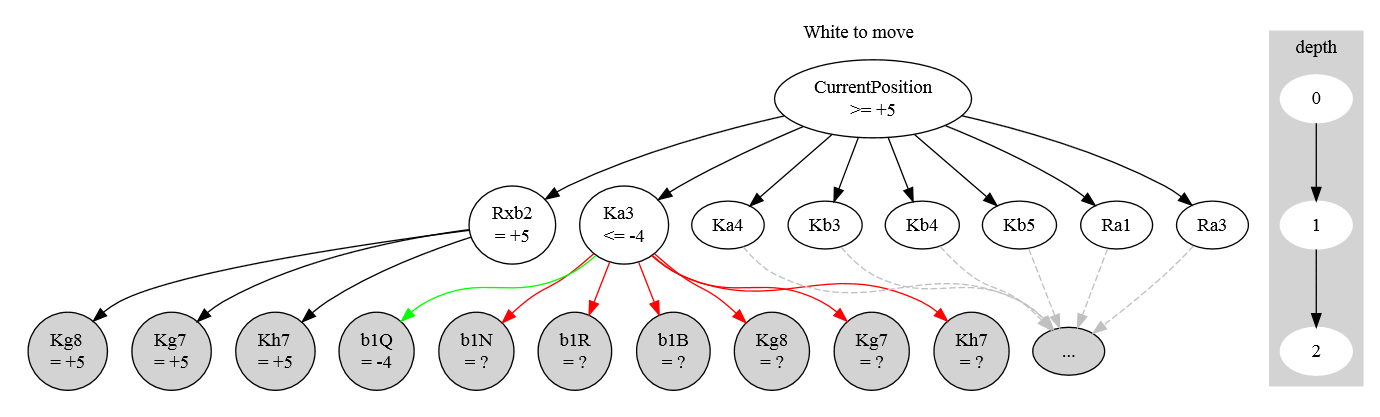
\includegraphics[width=\textwidth]{images/theory/AlphaBetaExample2.png}
    \caption[Beispielhafter Spielbaum der Tiefe 2 inklusive Evaluation]{Beispielhafter Spielbaum der Tiefe 2 inklusive Evaluation}
    \label{fig:alpha-beta_game-tree}
\end{figure}

Die Ausgangssituation sieht wie folgt aus:

\newgame
\def\AlphaBetaStart{kh8, pb2, Ra2, Ka4}
\def\AlphaBetaRxb{kh8, Rb2, Ka4}
\def\AlphaBetaKa{kh8, Ra2, Ka3,qb1}
\setchessboard{setpieces=\AlphaBetaStart}
\begin{center}
    {\chessboard[largeboard]}
\end{center}

Zunächst wird der Zug Rxb2 analysiert, auf den Schwarz mit drei Zügen reagieren kann (Kg8, Kg7 oder Kh7).
Nun sind wir in der maximalen Tiefe angekommen und deshalb werden Kg8, Kg7 und Kh7 der Reihe nach statisch evaluiert.
Dies führt jeweils zu einem Wert von +5, denn Weiß hat in allen drei Variationen einen extra Turm.

\setchessboard{setpieces=\AlphaBetaRxb, mover=b}
\begin{center}
    \chessboard[largeboard,pgfstyle=straightmove, markmove={h8-g8,h8-g7,h8-h7}]
\end{center}

Jetzt kann man Alpha mit einem Wert von +5 belegen, denn falls Weiß möchte, kann es den Zug Rxb2 spielen und sich eine Evaluation von +5 garantieren.

Anschließend wird der zweite Zug Ka3 analysiert.
Schwarz hat sieben Möglichkeiten auf Ka3 zu antworten (b1Q, b1R, b1N, b1B, Kg7, Kh7, Kg8).
Da wir wieder die Tiefe zwei erreicht haben, werden die Züge statisch evaluiert.
Die Analyse des ersten Zugs b1Q führt zu einer Evaluation von -4, denn Schwarz hat nun eine Dame für weiß' Turm (im Graph mit grünem Pfeil gekennzeichnet).

\setchessboard{setpieces=\AlphaBetaKa, mover=w}
\begin{center}
    \chessboard[largeboard,pgfstyle=straightmove, markmove={b2-b1}]
\end{center}

Aus dieser Erkenntnis können wir schließen, dass aus Ka8 höchstens eine Position mit der Evaluation von -4 resultiert, da Schwarz der minimierende Spieler ist.
Alpha, die Evaluation die der maximierende Spieler Weiß auf jeden Fall erreich kann, beträgt jedoch bereits +5.
Deshalb steht fest, dass Weiß Ka3 nicht spielen wird und die restlichen sechs möglichen Züge von Schwarz brauchen auch nicht mehr evaluiert zu werden (im Graph mit roten Pfeilen gekennzeichnet).

Ähnlich wie in diesem Beispiel, würde auch ein menschlicher Spieler in dem meisten Situationen wohl kaum Zeit dafür verwenden, einen Zug zu analysieren, der dem Gegner eine extra Dame ermöglicht [\cite{Paulsen2009}].

Um die Alpha-Beta-Suche zu implementieren, wird eine weitere Methode benötigt, die nach der Erkenntnis, dass sich das Fortsetzen der Analyse des Teilbaums nicht weiter lohnt, den Algorithmus für diesen Teilbaum stoppt.
Hierfür wird der Pseudocode aus dem Kapitel Minimax mit den beiden beschriebenen Variablen Alpha und Beta erweitert.
Diese werden zu Beginn mit den jeweils schlechtmöglichsten Werten für Weiß und Schwarz belegt ($-\infty$ und $\infty$) und den Prozeduren Minimize (Algorithmus~\ref{alg:alpha-beta_minimize}) und Maximize (Algorithmus~\ref{alg:alpha-beta_maximize}), wie die Tiefe, als Argument übergeben.

\begin{algorithm}
    \caption{MAXIMIZE Funktion}
    \label{alg:alpha-beta_maximize}
    \begin{algorithmic}[1]
        \Function{maximize}{Integer $d$, Position $p$, Float $alpha$, Float $beta$}
        \If{$d < 1$}
        \State \Return evaluate($p$)
        \Else
        \State $score \gets -\infty$
        \State $legalMoves \gets findLegalMoves(p)$
        \ForAll {$m$ in $legalMoves$}
        \State p.move(m)
        \State $moveScore \gets minimize(d-1, p, alpha, beta)$
        \State p.undoMove(m)
        \If{$moveScore > score$}
        \State $score \gets moveScore$
        \EndIf
        \If{$score >= beta$}
        \State break
        \EndIf
        \EndFor
        \EndIf
        \State \Return $score$
        \EndFunction
    \end{algorithmic}
\end{algorithm}

\begin{algorithm}
    \caption{MINIMIZE Funktion}
    \label{alg:alpha-beta_minimize}
    \begin{algorithmic}[1]
        \Function{minimize}{Integer $d$, Position $p$, Float $alpha$, Float $beta$}
        \If{$d < 1$}
        \State \Return evaluate($p$)
        \Else
        \State $score \gets \infty$
        \State $legalMoves \gets findLegalMoves(p)$
        \ForAll {$m$ in $legalMoves$}
        \State p.move(m)
        \State $moveScore \gets maximize(d-1, p, alpha, beta)$
        \State p.undoMove(m)
        \If{$moveScore < score$}
        \State $score \gets moveScore$
        \EndIf
        \If{$score <= alpha$}
        \State break
        \EndIf
        \EndFor
        \EndIf
        \State \Return $score$
        \EndFunction
    \end{algorithmic}
\end{algorithm}
\newpage
